% -*- mode: fundamental -*-

% Pre-tutorial placeholder for Slides for 2-hour tutorial
%   at RISC-V Summit, Oct 22, 2025, Santa Clara
% Title: "Learn to Design and Verify a 6-stage pipelined RISC-V CPU"

% Copyright (c) 2025 Rishiyur S. Nikhil, All Rights Reserved

% -*- mode: fundamental -*-

% Copyright (c) 2025 Rishiyur S. Nikhil, All Rights Reserved

% Preamble that is shareable across slide decks

\documentclass[10pt, aspectratio=169]{beamer}

% \documentclass[17pt]{beamer}

% Avail. font sizes: 8pt, 9pt, 10pt, 11pt, 12pt, 14pt, 17pt, 20pt.
% Default font size is 11pt (= 22pt in full screen mode).

\usepackage{verbatim}
\usepackage{fancyvrb}

% ================================================================
% Themes

\usetheme{Madrid}          % Line at bottom: Author (affiliation), OptTitle, Conf, page 

% \usetheme{Copenhagen}    % Same as Madrid except bottom line: Author, OptTitle

% \usetheme{Berkeley}    % Takes up 1-inch border on left and top

% ----------------
% colorthemes
% (default), beaver, beetle, seahorse, wolverine

\usecolortheme{seahorse}

% ================================================================
% Customization: show table of contents before each section
% Use \AtBeginSubsection    to show before each subsection

% \AtBeginSection[]
% {
%   \begin{frame}
%     \frametitle{Table of Contents}
%     \tableofcontents[currentsection]
%   \end{frame}
% }

% ================================================================

% ----------------
% ITALICISE WORDS
\newcommand{\ie}{\emph{i.e.,}}
\newcommand{\eg}{\emph{e.g.,}}
\newcommand{\Eg}{\emph{E.g.,}}
\newcommand{\etc}{\emph{etc.}}
\newcommand{\via}{\emph{via}}
\newcommand{\vs}{\emph{vs.}}

% ----------------
% EMPTY BOXES OF VARIOUS WIDTHS, FOR INDENTATION
\newcommand{\hm}{\hspace*{1em}}
\newcommand{\hmm}{\hspace*{2em}}
\newcommand{\hmmm}{\hspace*{3em}}
\newcommand{\hmmmm}{\hspace*{4em}}

% ----------------
% Convenient widths

\newlength{\hlessmmm}
\setlength{\hlessmmm}{\textwidth}
\addtolength{\hlessmmm}{-3em}

\newlength{\hlessmmmm}
\setlength{\hlessmmmm}{\textwidth}
\addtolength{\hlessmmmm}{-4em}

% ----------------
% STRUTS
% HORIZONTAL STRUT.  One argument (width).
\newcommand{\hstrut}[1]{\hspace*{#1}}
% VERTICAL STRUT. Two arguments (offset from baseline, height).
\newcommand{\vstrut}[2]{\rule[#1]{0in}{#2}}
% ----------------
% ``TIGHTLIST'' ENVIRONMENT (no para space betwee items, small indent)
\newenvironment{tightlist}%
{\begin{list}{$\bullet$}{%
    \setlength{\topsep}{0in}
    \setlength{\partopsep}{0in}
    \setlength{\itemsep}{0in}
    \setlength{\parsep}{0in}
    \setlength{\leftmargin}{1.5em}
    \setlength{\rightmargin}{0in}
    \setlength{\itemindent}{0in}
}
}%
{\end{list}
}
% ----------------

% End of preamble
% ****************************************************************


\newcommand{\bsc}{\emph{bsc}}
\newcommand{\BSV}{\bf BSV}
\newcommand{\Drum}{\bf Drum}
\newcommand{\Fife}{\bf Fife}
\newcommand{\TestRIG}{\bf TestRIG}
\newcommand{\BookRepo}{\url{https://github.com/rsnikhil/Learn_Bluespec_and_RISCV_Design}}

% Note: font sizes: \small > \footnotesize > \scriptsize > \tiny

% ****************************************************************
% Title page

\title[Design \& Verify 6-stage RISC-V CPU]
      {Learn to Design and Verify a 6-stage pipelined RISC-V CPU}

% \subtitle{foo\rule[0in]{0in}{4ex}}

\author[{\copyright} R.S.Nikhil]{Rishiyur S.~Nikhil, Cofounder and CTO, Bluespec, Inc.}

% \institute{Bluespec, Inc.}

\date{October 22, 2025}

% ****************************************************************

\begin{document}

% ****************************************************************
% ****************************************************************
% ****************************************************************

\begin{frame}[fragile]
 \titlepage

 \begin{center}
  {\small Tutorial at Developer's Day, RISC-V Summit, Santa Clara CA}

  
\includegraphics[height=1cm]{Figures/Bluespec_Logo_2022-10}
 \end{center}
\end{frame}

% ****************************************************************
% ****************************************************************
% ****************************************************************

\begin{frame}[fragile]

\begin{center}

  \vstrut{0em}{10ex}

  {\LARGE PLACEHOLDER}

  \vspace*{10ex}

  \begin{minipage}{0.7\textwidth}
    This is a placeholder for the slide deck which will be used at the tutorial.

  \vspace*{5ex}

    It will be replaced by the final slide deck shortly before the
    actual tutorial on October 22, 2025.
  \end{minipage}

\end{center}

\end{frame}

% ================================================================

\begin{frame}[fragile]
\frametitle{The Plan for Today}

\begin{center}
 \begin{minipage}{0.55\textwidth}\scriptsize
  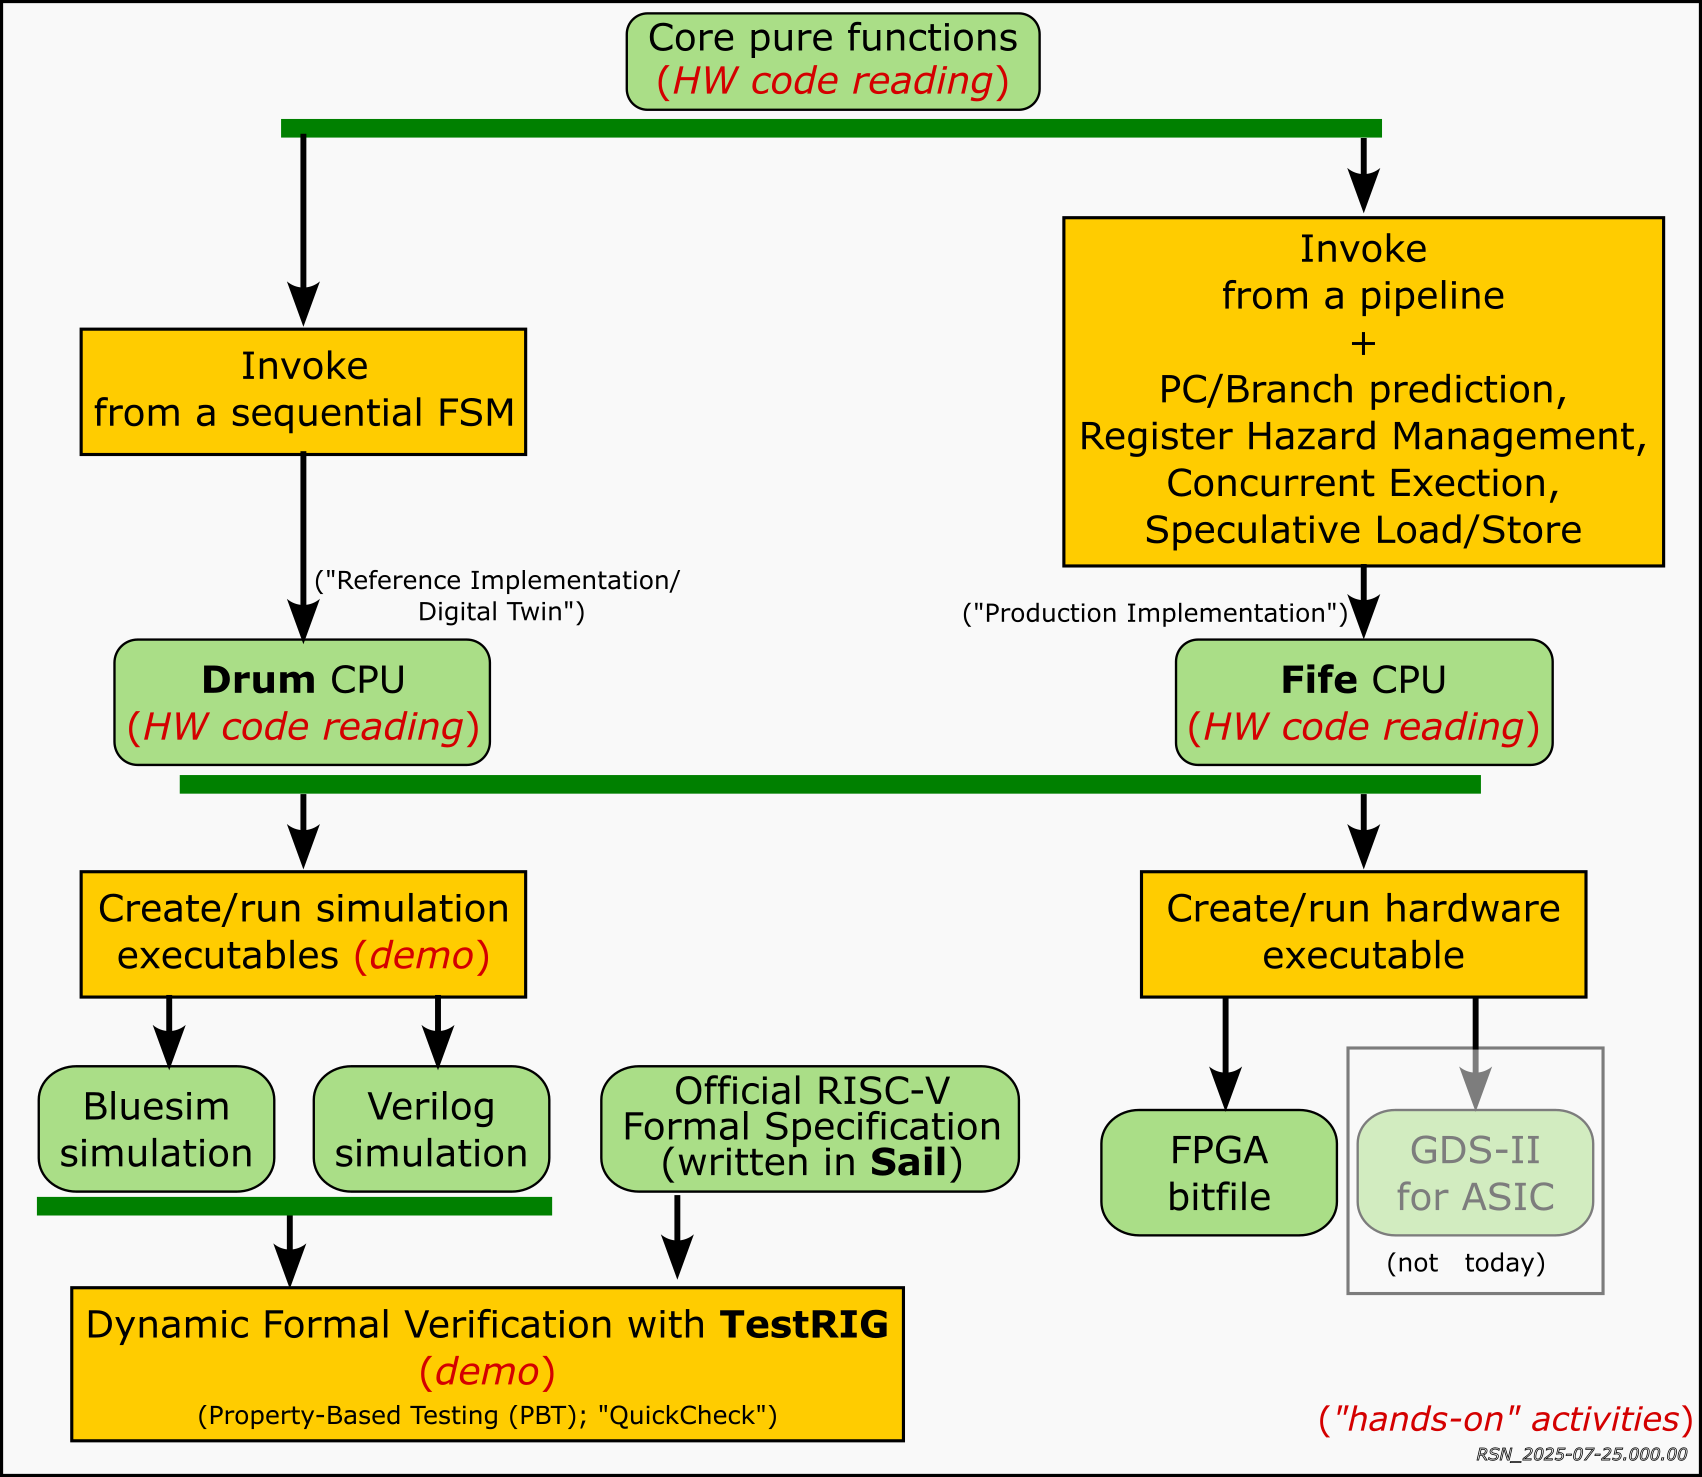
\includegraphics[height=0.87\textheight]{Figures/RSN_2025-07-25.000.00_Tutorial_Plan.png}
 \end{minipage}
 \begin{minipage}{0.44\textwidth}\scriptsize

  ``Hands on'':
  \begin{itemize}
   \item We will read the code together
   \item We create and run simulation executables together
   \item We will verify the design together
  \end{itemize}
  {\tiny (If you haven't installed the tools yet, please just listen
  and follow; hopefully you will try everything on your own, later)}

  \vspace{5ex}

  Not ``Hands on'' (lecture and demo only):
  \begin{itemize}
   \item How to build and run on FPGA
  \end{itemize}

  \vspace{5ex}

  ``But I'm not familiar with hardware design'' or \\ ``I'm not familiar
  with the language used'' ...

  \hm ... don't worry:
  \begin{itemize}
   \item For "Core pure functions" and {\Drum}, the code looks just like
         a conventional programming language

   \item {\Fife} will introduce pipelining and pipeline techniques; we
         will explain the code in more detail.
  \end{itemize}
 \end{minipage}
\end{center}

\end{frame}

% ================================================================

\begin{frame}[fragile]

\frametitle{Prerequisites}

\begin{center}\scriptsize
 \begin{minipage}{0.9\textwidth}
  We \emph{do} assume that you are familiar with:
  \begin{itemize}

   \item Some ISA (Instruction Set Architecture): Machine Instructions
     and/or assembly-language (RISC-V or other).

     \vspace*{1ex}

     We're not going to explain what is a general-purpose register,
     what is a Program Counter, what is an arithmetic instruction,
     what is a BRANCH or JAL/JALR instruction, what is a LOAD/STORE
     instruction, etc.; we're assuming you already know these things.

   \vspace*{1ex}

   \item General coding (in C, Python, Go, Rust, Haskell, Verilog,
     SystemVerilog, ... whatever), so you can quickly grasp new,
     unfamiliar code.

     Familiarity with enum and struct types, functions, if-then-else.

     General knowledge of object-oriented programming is useful.
  \end{itemize}

  \vspace*{5ex}

  We \emph{do not} assume that you are familiar with:
  \begin{itemize}

   \item Hardware design, or any hardware design language (Verilog,
     SystemVerilog, Bluespec BSV or BH, Chisel, ...)

   \item Pipelined micro-architecture of CPUs

  \end{itemize}

  \vspace*{5ex}

  On the Tutorial Web Page
    (\url{https://github.com/rsnikhil/Tutorial_RISCV_Summit_2025}),
    we've asked you to install certain tools so that you can examine
    code and build and run things along with me during this tutorial.

  \vspace*{2ex}

  If you haven't done this already, then please just sit back and
  follow the lecture and demos, for now.  We hope that you will be
  motivated to later install the tools and try everything out for
  real.

 \end{minipage}
\end{center}

\end{frame}

% ****************************************************************
% ****************************************************************
% ****************************************************************

\end{document}
